\documentclass[notitlepage]{scrreprt}

\usepackage{fancyhdr}
\usepackage[english]{babel}
\usepackage{ucs}
\usepackage[utf8x]{inputenc}
\usepackage[bookmarksopen=true,
	bookmarks=true,
	plainpages=false,
	pdfpagelabels=true,
	colorlinks=true,
	linkcolor=black,
	citecolor=black,
	filecolor=black,
	urlcolor=blue]{hyperref}
\usepackage{graphicx}
\usepackage{float}
\usepackage{listings}
\usepackage{color}
\usepackage{tikz}
\usepackage{amsmath}

\lstdefinestyle{MyCStyle}{
  belowcaptionskip=1\baselineskip,
  breaklines=true,
  frame=single,
  captionpos=b,
  numbers=left,
  xleftmargin=\parindent,
  language=C,
  showstringspaces=false,
  basicstyle=\footnotesize\ttfamily,
  keywordstyle=\bfseries\color{green!40!black},
  commentstyle=\itshape\color{purple!40!black},
  identifierstyle=\color{blue},
  stringstyle=\color{orange}
}
\lstset{escapechar=@,style=MyCStyle}

\pagestyle{fancy}
\fancyhf{}
\fancyhead[R]{Heart Rate Monitor}
\fancyhead[L]{Fabian Meyer, Jens Gansloser}
\fancyfoot[C]{\thepage}

\fancypagestyle{plain}{%
    \fancyhf{}
	\fancyhead[R]{Heart Rate Monitor}
	\fancyhead[L]{Fabian Meyer, Jens Gansloser}
	\fancyfoot[C]{\thepage}
}

\begin{document}

\title{Heart Rate Monitor}
\subtitle{Ubiquitous Computing Mini Project}
\author{Fabian Meyer \and Jens Gansloser}
\date{\today \\ HTWG Konstanz}
\maketitle
\thispagestyle{empty}

\begin{figure}[H]
	\centering
	
\includegraphics[width=150px]{images/htwgLogo.jpg}
\end{figure}

\begin{abstract}
The aim of this project is to build a heart rate monitor (HRM) device. There are already a lot of devices commercially available which measure the heart rate. However, the internal functionality of these devices is not exposed to the user, so there cannot be made any statements about their precision and the quality of the results. Additionally, most devices need to be worn on the users chest or the user must place his finger on it. This document describes the principle and implementation of a heart rate monitor device, which is able to detect the heart rate with high precision and can be worn as a wrist band.
\end{abstract}
\clearpage

\tableofcontents

\chapter{Principle of Operation}
\label{chap:principle-of-operation}

There are several ways to measure the heart rate. For this project, a technique is required which uses small and cheap hardware and can be used mobile. Also the performance requirements should be low, to allow an implementation with small energy-saving micro controllers. This chapter describes the method used for HRM to get the heart rate.

\section{Heart Rate}
A method to measure the heart rate is the photoplethysmogram (PPG) technique. This method measures the change of the blood volume through the absorption or reflection of light. A light emitting diode (LED) shines through a thin amount of tissue (e.g. fingertip, earlobe). The wavelength of the light should be in near infra-red area. On the other side a photo-diode registers the intensity of light that traversed the tissue. Since blood changes its volume with each heart beat, more or less light of the LED gets absorbed by it. If the heart pushes blood through the vessels, more blood flows between the LED and photo-diode (it has a higher volume) and more light is absorbed by it. That means less light is registered by the photo-diode. If blood flows from the vessels to the heart, less light is absorbed by it (the volume declines) and the photo-diode detects more light. As a result the registered intensity of light changes continuously with the pulse. By measuring the time between two intensity peaks the current pulse can be estimated. The setting for the pulse rate monitor is displayed in figure \ref{fig:pulse-rate-monitor-setting}.

\begin{figure}[H]
	\centering
	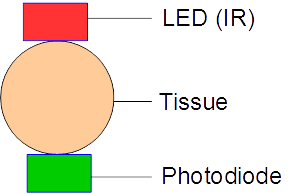
\includegraphics[width=180px]{images/pulse-rate-aufbau.png}
	\caption{Pulse Rate Monitor Setting - Light through skin}
	\label{fig:pulse-rate-monitor-setting}
\end{figure}

\newpage

An alternative way to measure the heart rate with the same technique is to detect the reflected light. The LED and the photo-diode can be placed on the same side. This setting is displayed in figure \ref{fig:pulse-rate-monitor-setting2}

\begin{figure}[H]
	\centering
	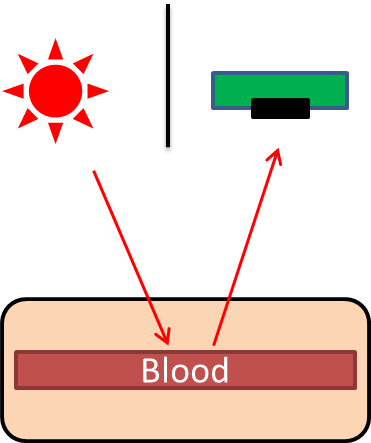
\includegraphics[width=130px]{images/pulse-rate-aufbau2.png}
	\caption{Pulse Rate Monitor Setting - Light reflected}
	\label{fig:pulse-rate-monitor-setting2}
\end{figure}

Based on these two techniques, the application offers high flexibility to the kind of measurement. The heart rate can be measured through the fingertip, at the ear or at other places. For the prototype, the measurement principle with the fingertip is used. 

\section{Oxygen Saturation}
The oxygen saturation of the blood can be measured by using 2 light emitting diodes. One LED emits light with a wavelength of 660nm (red light), the other emits light with a wavelength of 940nm (infra-red light). The absorption of light by blood changes corresponding to its oxygen saturation. Oxygenated blood absorbs more infra-red light and less red light. With de-oxygenated blood it is the other way around \cite{bib:pulse-oximetry}. The LEDs blink alternating and a photo-diode is used to measure the light intensity after the light traversed the tissue. These measurements in combination with the Lambert-Beer-Law are used to calculate the oxygen saturation.

\chapter{Environment}
\label{chap:environment}
This chapter describes the hardware and the software used and implemented for the project. Figure \ref{fig:data-flow} shows the different hardware parts and how they interact with each other. Note that the displayed setting is different from the actual used one in the prototype due to wrong hardware orders. The prototype setting is explained in chapter \ref{chap:hrm}.

\begin{figure}[H]
	\centering
	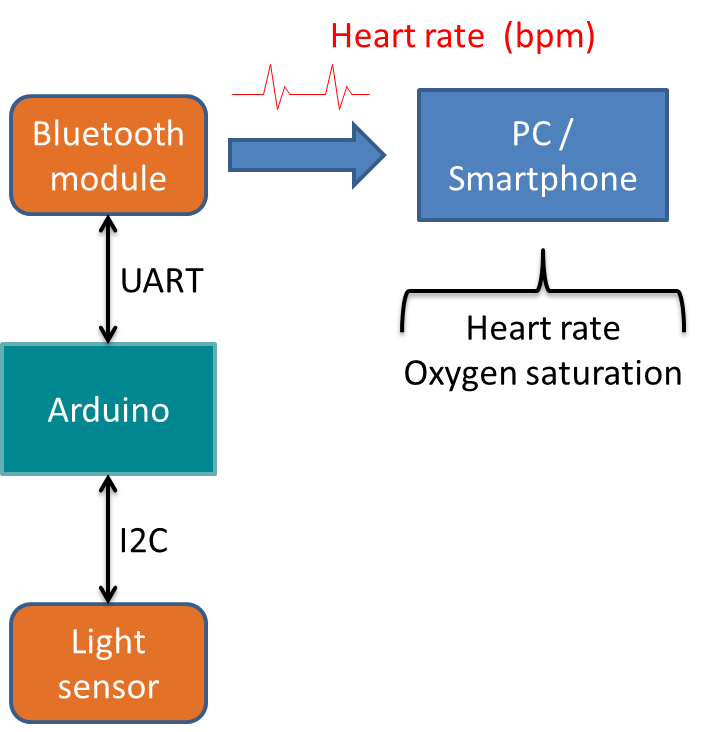
\includegraphics[width=200px]{images/general_dataFlow.png}
	\caption{Project setup}
	\label{fig:data-flow}
\end{figure}

\section{Hardware}
\subsection{Light Intensity Sensor}
To measure light, the 16bit TSL2561 Luminosity Sensor breakout board from Adafruit is used. It provides the TSL2561 Light-To-Digital Converter which is able to sense full spectrum and IR light with a very high sensitivity (see figure \ref{fig:tsl-2561-spectrum}). The sensor contains a broadband photo-diode (visible and infra-red) and a infra-red photo-diode. Two ADCs convert the analog data to digital data, that can be read via the I$^{2}$C bus. The light sensor can be configured with different gain, which changes its sensitivity to light. This is required if the sensor is used in areas with bright or low environment light. A second option to configure is the integration time (13ms, 101ms, 402ms). This configures the resolution of the device, so that the sensor has more time to take samples. With a integration time of 402ms, the sensor has the complete 16bit resolution. The output of the sensor can be used to calculate the measured SI-Unit lux, which indicates the illuminance \cite{bib:tsl-sensor}. Figure \ref{fig:tsl-2561-spectrum} shows the light spectrum of the two photo-diodes on the board.

\begin{figure}[H]
	\centering
	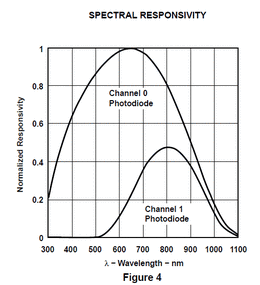
\includegraphics[width=200px]{images/light_tsl2561spectrum.png}
	\caption{TSL-2561 Spectrum}
	\label{fig:tsl-2561-spectrum}
\end{figure}

\subsection{Microcontroller}
The data of the sensor is further computed by an Arduino \cite{bib:arduino-board}. The Arduino receives the data from the light sensor via the I$^{2}$C bus system. Different Arduinos can be used. The only requirements to the Microcontroller are I$^{2}$C and UART (for Bluetooth/serial) interfaces to communicate with the light sensor and the PC/Smartphone.

\subsection{Bluetooth Module}
The Bluefruit EZ-Link is a serial link bluetooth module. That means, the Arduino can communicate via UART with the bluetooth module, which handles the wireless transmission to the computer/smartphone. On the computer side, the module (if it was paired successfully) is recognized as an serial port. See also \cite{bib:bluetooth-adapter}.

\newpage

\section{Libraries}
To create the heart rate monitor, several external libraries were used. This section lists all used external libraries and explains its usage.

\subsection{FFTW}
FFTW is a C library, which offers functions to calculate the discrete Fourier Transform (DFT). It supports the calculation with multiple dimensions, complex or real data and different input sizes. HRM uses FFTW to compute the complex DFT of the light sensors signal and determine the heart rate.

\subsection{Qt}
Qt is a cross-platform C++ library for creating Graphical User Interfaces (GUIs). Additionally, it supports own container classes, networking, database access and a lot of more. For the HRM, Qt is used to create the GUI.

\subsection{Qwt}
Qwt is an add-on for Qt which is able to create 2D and 3D plots. Its advantages are the large amount of features and the high performance. This makes it suitable for technical applications, which need to display a lot of data. Qwt is used to plot the light sensors data and its Fourier Transformed.

\subsection{QtSerialPort}
QtSerialPort is used to access the serial port from the PC. It is an add-on module for Qt4 and Qt5. It allows fast and easy writing and reading to/from the serial ports. Because Qt is used for the Graphical User Interface (GUI), this is the optimal solution for serial port access.

\subsection{Light Intensity Sensor Driver}
To get data from the light sensor, the Adafruit TSL2561 and Adafruit Unified Sensor Driver libraries are used. These libraries do the I$^{2}$C communication and the digital to lux calculation. Also they provide functions to set the gain and integration time \cite{bib:tsl-library} \cite{bib:sensor-library}.

\newpage

\section{Heart Rate Monitor Software}
This section shows all implemented modules which are part of HRM. The implementation details are outlined in chapter \ref{chap:impl-details}. The software for the PC-part is implemented in C++. CMake is used as build-tool. The Arduino part is developed with the Arduino IDE. The application is cross-platform capable and supports Qt4 and Qt5. Compilation was tested on Linux and Windows.

\subsection{Graphical User Interface}
The GUI is mainly used for debugging and optimization. The GUIs features are shown in the following list:

\begin{itemize}
	\item{Displays the received data from the Arduino (via serial port)}
	\item{Displays the light sensors settings}
	\item{Allows setting of the light sensors sample rate}
	\item{Displays several diagrams (sensor values, frequency spectrum, ...)}
	\item{Displays the signal processing parameter}
\end{itemize}

\subsection{Serial Interface}
The class \lstinline{Serial} is used to control the access to the serial port. Qts slot and signal mechanism is used, to notify other classes when data is received. The class supports sending and receiving data. 

\subsection{Signal Processing Module}
This is the main part of HRM. It is responsible for detecting the heart rate. The class \lstinline{FFT} executes all signal processing steps explained in chapter \ref{sec:signal-processing}.

\subsection{Arduino Module}
The Arduino software is executed on the Arduino board. It controls the light sensor and sends its data via UART to the PC. It uses the extended Adafruit driver to allow manual timing (using own sample rates). Additionally to that, it is able to parse incoming serial data: The light sensors settings can be queried, also a command to set the sample rate is available.

\newpage

\subsection{Extended Light Intensity Sensor Driver}
The TSL2561 driver was extended to allow manual timing. Manual timing is required to allow custom sample rates. The standard driver allows only pre-configured sample rates, although the TSL2561 controller does support manual timing. Because the signal processing requires configurable sample rates, the driver was extended to allow this feature.\\

\subsection{Overview}
Figure \ref{fig:software} summarizes the previously outlined software.

\begin{figure}[H]
	\centering
	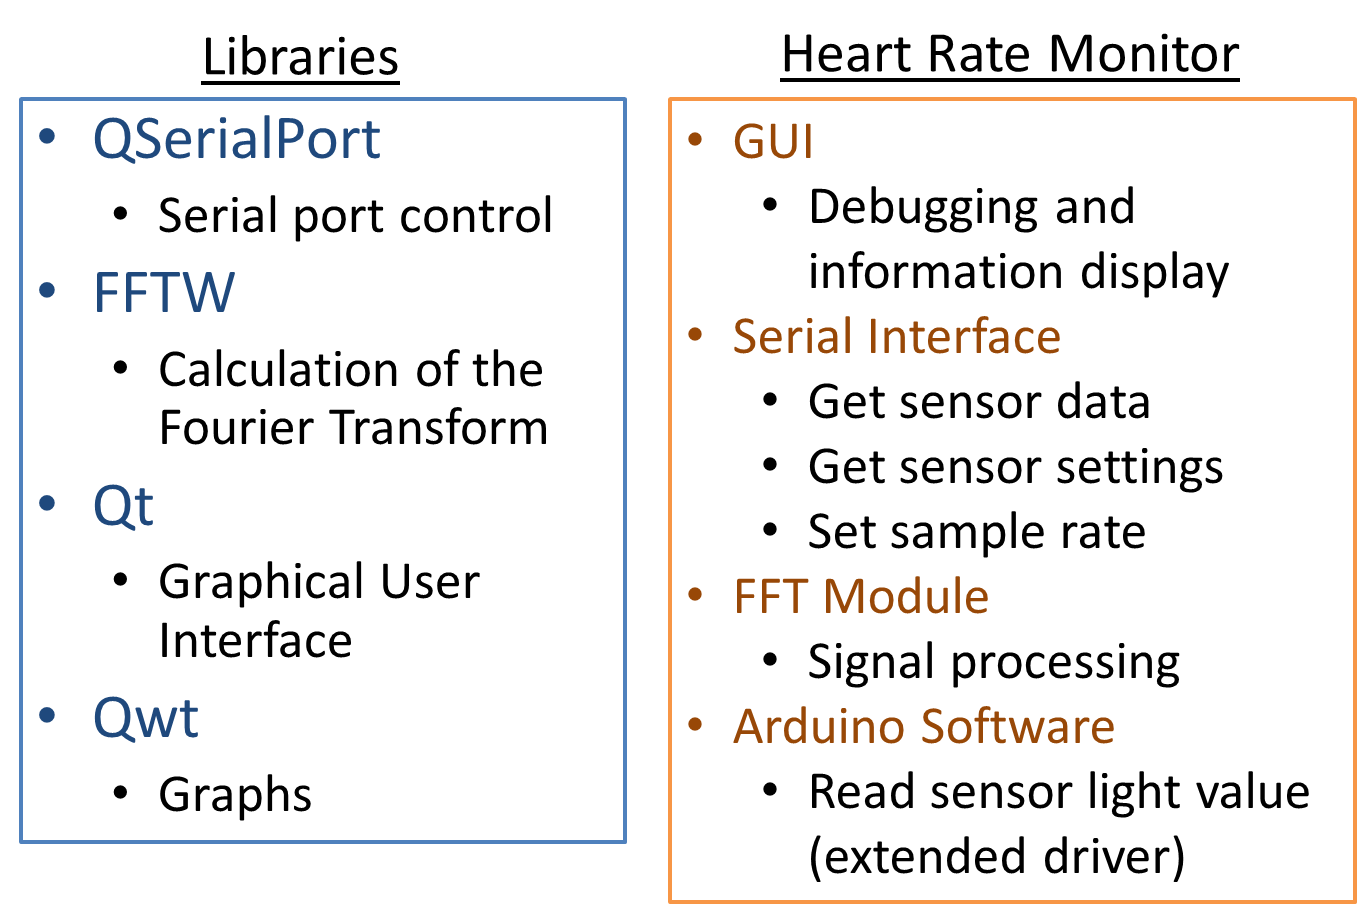
\includegraphics[width=250px]{images/software.png}
	\caption{HRM Software}
	\label{fig:software}
\end{figure}

\chapter{Heart Rate Monitor}
\label{chap:hrm}
\section{Solution Approach}
Figure \ref{fig:raw-data} shows the output signal from the light sensor. The diagram shows the different luminosity values over time (= heart rate) of a patient. It is measured by placing the finger between the light sensor and the LED.

\begin{figure}[H]
	\centering
	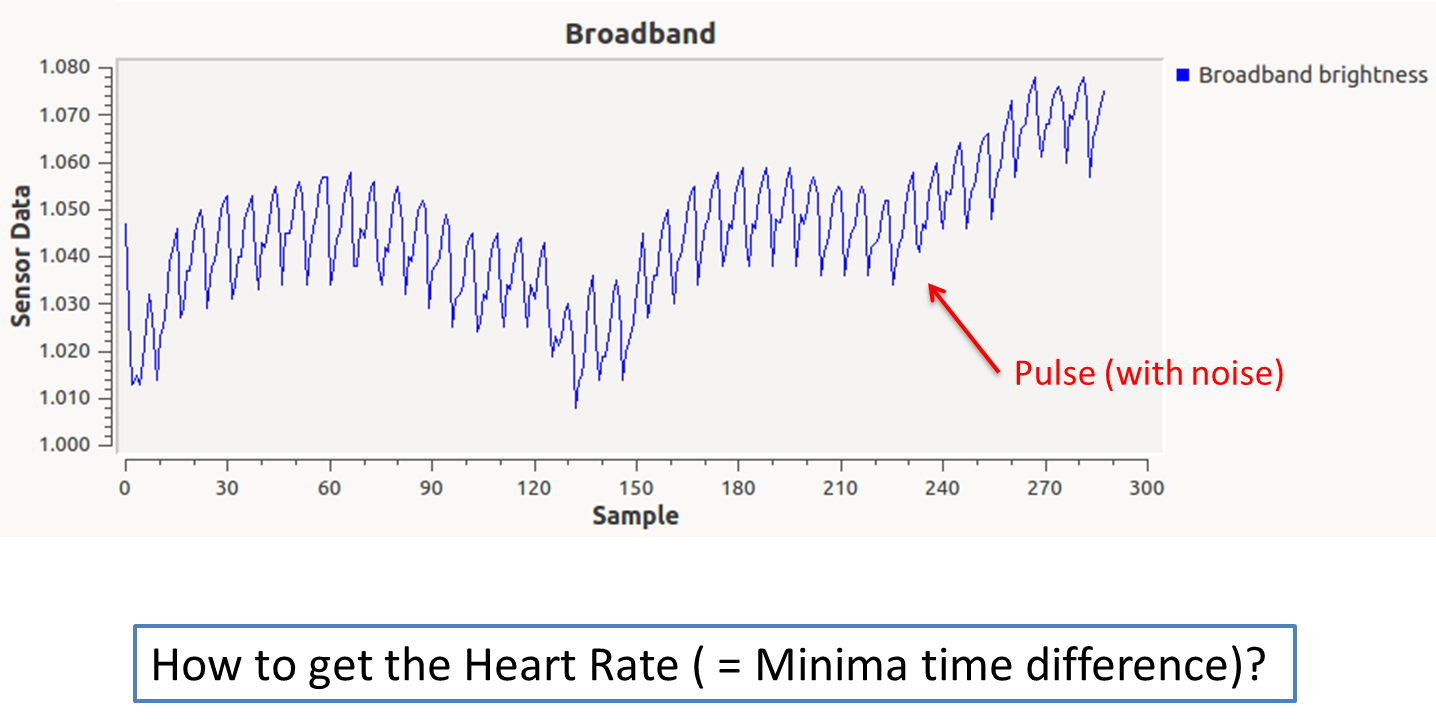
\includegraphics[width=300px]{images/rawData.png}
	\caption{Raw light sensor data}
	\label{fig:raw-data}
\end{figure}

To get the exact heart rate, the time between two minima (or maxima) of the discrete sensor values need to be determined. However, it is not trivial to determine the minima, because of the noise in the signals data. The noise comes from different environment settings, the difference in blood volume change of each person and how the finger is placed onto the sensor. These parameter result in a change in the data's y-part.

\subsection{First Approach}
A first naive approach is to determine the grade of each two sample points in the input data and identify if the curve is declining or rising. With this knowledge, the minima could be identified. However, this approach is not optimal. It is impossible to separate different minima in the data and find the correct ones. Due to the noise local minima could be detected which are not required. Introducing a static limit is unsuitable too, because in the difference of the y-axis data in each sample. To conclude, this approach is not suitable for the problem.

\subsection{Second Approach}
As one can see in figure \ref{fig:raw-data}, the heart rate is represented by a periodic up and down of the input values. These up and down values are distorted by some noise. The time difference between two minimas can also be expressed as the frequency of these periodic curve. Viewed from a signal processing view, these up and downs have the highest contribution of frequencies to the input signal. To get the heart rate, the frequency which contributes most to the input signal (= heart rate) has to be determined. This is a perfect application field for the Fourier Transform. The Fourier Transform is a mathematical method to analyse an input signal and determine the different frequencies which contribute how much to this signal. A Fourier Transform converts an input signal in the time domain to an output signal in the frequency domain (the frequency spectrum). The output signal shows, how much each frequency contributes to the input signal. The basic idea is, to transform the input signal via the Fourier Transform and then determine the signal which contributes most. This means determining the peak of the output frequency signal. Picture \ref{fig:basic-operation} shows the basic operation principle.

\begin{figure}[H]
	\centering
	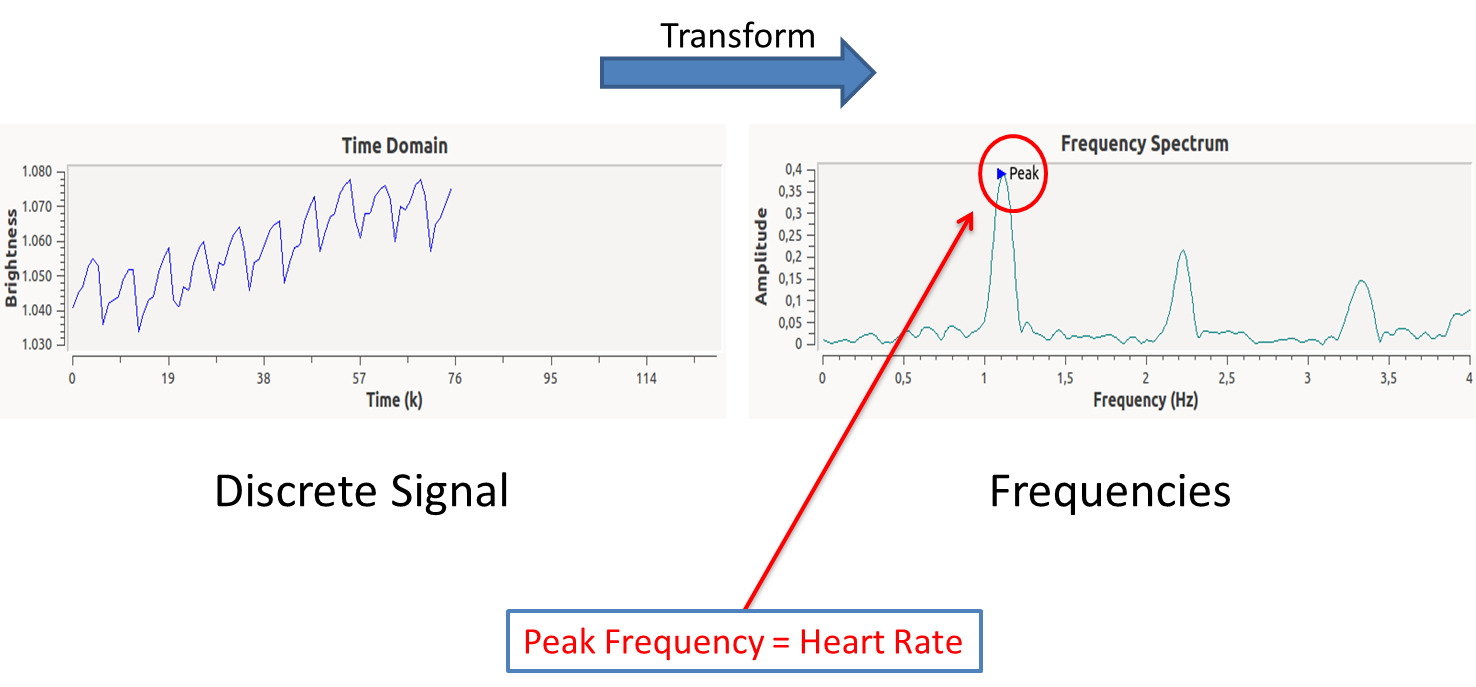
\includegraphics[width=400px]{images/basicOperation.png}
	\caption{Basic Operation principle}
	\label{fig:basic-operation}
\end{figure}

\section{Data Flow}
To implement HRM, at first a data flow design has to be created. Because the implementation of the signal processing is not trivial and the debugging capabilities on the Arduino are limited, the first prototype is created on a PC. The data flow between Arduino and light sensor via $I^2C$ can be separated in a control and application part. The control part contains the configuration of the sensor (setting configuration from Arduino to sensor). The application part contains the luminosity values (reading from sensor to Arduino). Like the $I^2C$ communication, the UART communication can be separated in control and application flow, too. For the application part, the Arduino sends the luminosity values to the PC. The control part consist of setting the sample rate of the sensors data or querying for the sensors settings from the PC. The PC collects the sensors values. When enough samples are collected, it executes the signal processing to identify the heart rate. Figure \ref{fig:data-flow2} shows the hardware set-up used in the prototype. At the moment, HRM can detect the heart rate. It can be easily extended to measure the oxygen saturation.

\begin{figure}[H]
	\centering
	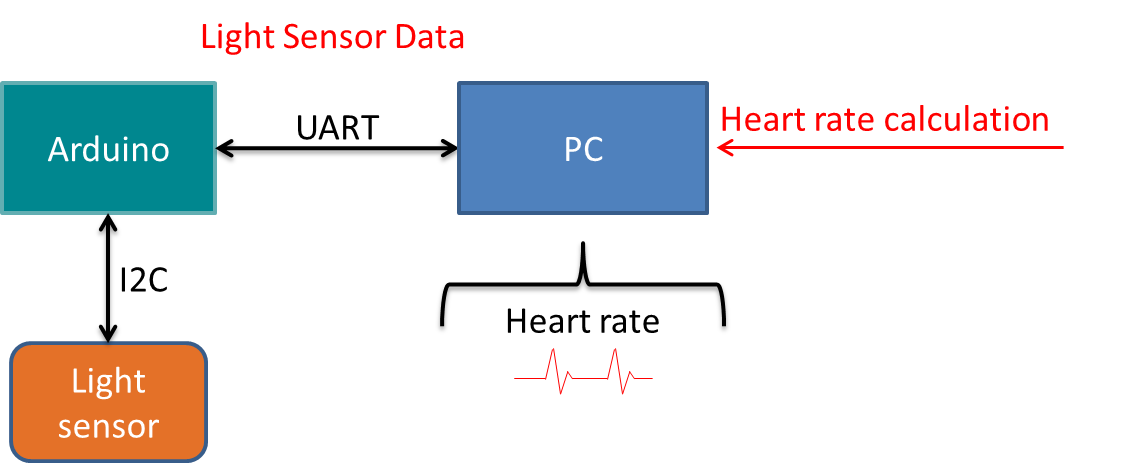
\includegraphics[width=350px]{images/general_dataFlow_second.png}
	\caption{Project Setup}
	\label{fig:data-flow2}
\end{figure}

\section{Signal Processing}
\label{sec:signal-processing}
This section describes the signal processing of the light sensors input values and how to identify based on this data the heart rate. The basic functionality and usage of the signal processing steps are explained. However, due to its complexity and its large scope, the derivation of the mathematical principles are not covered here.

\subsection{Fourier Transformation}
There are a lot of different kinds of Fourier Transforms (FT) for different application fields. First, the correct kind has to be determined.

\subsubsection{Synthesis or Analysis}
Fourier Transform can be used for analysis (forward FT) and synthesis (inverse FT). Because we want to get the frequency domain signal from the time domain signal, we use the forward transform (analysis).

\begin{figure}[H]
	\centering
	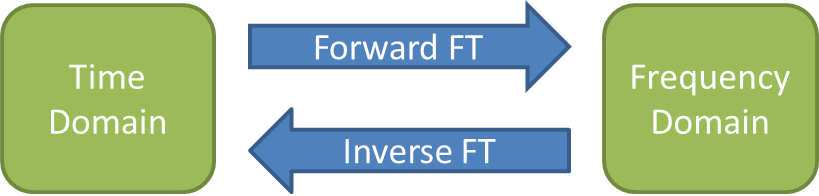
\includegraphics[width=200px]{images/DFT_types1.png}
	\caption{Synthesis or Analysis}
	\label{fig:dft-types1}
\end{figure}

\newpage

\subsubsection{Type of FT}
There are several different types of the FT, depending on the input signal. The following table explains the types and which FT to use.

\begin{table}[h]
\centering
\begin{tabular}{|l|l|}
	\hline
	\textbf{Input signal} & \textbf{FT type} \\ \hline
	Continues, aperiodic & Fourier Transform \\ \hline
	Continues, periodic & Fourier Series \\ \hline
	Discrete, aperiodic & Discrete Time Fourier Transform \\ \hline
	Discrete, periodic & Discrete Fourier Transform \\ \hline
\end{tabular}
\caption{FT types}
\end{table}

Because the input signal is an array of discrete values and it is finite, the discrete FT (DFT) is required. The input data is thought of it would be periodic, so the DFT instead of the DTFT is used (The DTFT is only used in theoretical signal analysis and uses infinite input data).

\subsubsection{Complex or Real}
The formula for the DFT is shown in \ref{fig:dft-formula}. Complex numbers are used. The input are complex discrete values $x[n]$. The output are complex discrete values $X[k]$. $N$ is the number of samples. The iterator $k$ represents the frequencies. Although there is a DFT with real values too, the complex DFT is used. The reason for that is that using this kind of transform is simply more common.

\begin{figure}[H]
	\centering
	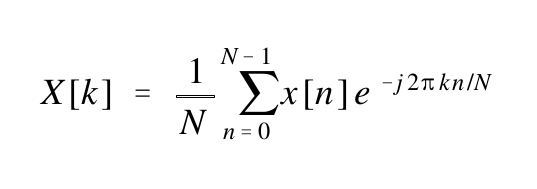
\includegraphics[width=250px]{images/complex_dft_formula.png}
	\caption{Complex DFT formula}
	\label{fig:dft-formula}
\end{figure}

An fast implementation of the DFT is the FFT. The FFTW library is used to compute the FFT of the sensors data. Also the FT is the basic principle to get the heart rate, additional steps need to be made to get a nice frequency spectrum. The following chapters describe the different steps in detail. Figure \ref{fig:signal-processing-steps1} shows the applied functions. The displayed frequency spectra in the following sections are all calculated with enabled zero padding. The result of disabling zero padding is shown in section \ref{subsec:zp}.

\begin{figure}[H]
	\centering
	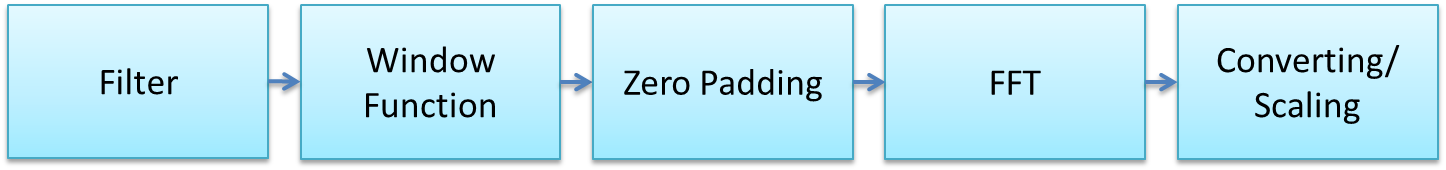
\includegraphics[width=350px]{images/signal_processing_steps1.png}
	\caption{Signal Processing Steps}
	\label{fig:signal-processing-steps1}
\end{figure}

\subsection{Filter}
Without applying the steps mentioned above, the output signal looks like shown in Figure \ref{fig:only-fft}. There are a lot of high Frequencies and it is difficult to find the correct optimum (Figure \ref{fig:basic-operation}, peak symbol). In the picture, the peak symbol points to the actual optimum. However, it is difficult to detect and not easy to find. The low frequencies are from the noise. To remove these unwanted frequencies, a bandpass filter is applied. To measure the heart rate, only heart rates from 40 - 230bpm are possible. This means, only frequencies from 0.7 - 3.9Hz need to be identified. All other frequencies in the input signal can be removed.

\begin{equation}
\begin{aligned}
40bpm \approx 0.7Hz\\
230bpm \approx 3.9Hz
\end{aligned}
\end{equation}

The bandpass filter allows only desired frequencies (a frequency range) and removes the remaining. The filter can be applied to the input signal (convoluting with e.g. butterworth bandpass filter) or to the output signal (multiplication - cutting the unwanted frequencies). When applying the filter before the FFT, it needs some time until it is stabilized. The stabilization time has to be cut off from the signal. Else, this would result in distorted output data. However, because the second option is much more faster and allows to use a perfect filter, this option is used. Using a perfect filter (rectangular function) is much more easier. It is not required to design the filter coefficients. Additionally, multiplying does not requires as much performance as convolution.

\begin{figure}[H]
	\centering
	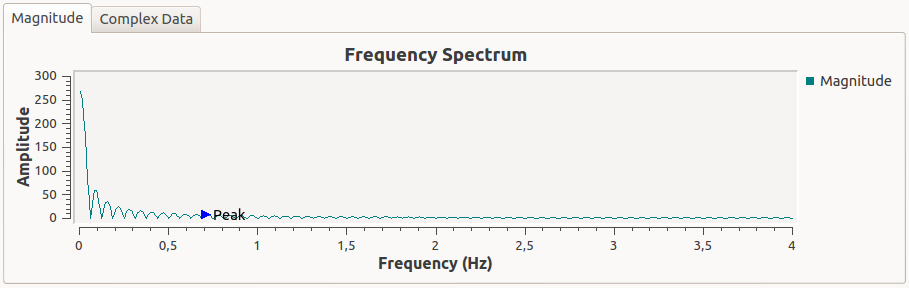
\includegraphics[width=350px]{images/OnlyFFTNoFilterAndWindow.png}
	\caption{Only FFT}
	\label{fig:only-fft}
\end{figure}

The frequency spectrum after applying the filter is shown in figure \ref{fig:filter}. The diagram does look much more better and the peaks are already good to detect.

\begin{figure}[H]
	\centering
	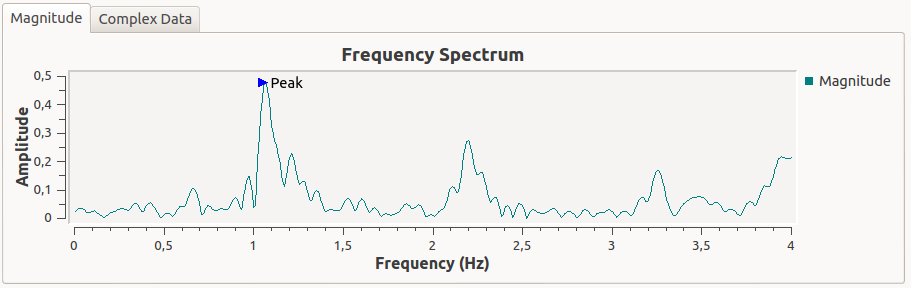
\includegraphics[width=350px]{images/withFilterNoWindow.png}
	\caption{With filter}
	\label{fig:filter}
\end{figure}

\subsection{Window Function}
Before executing the FFT, a window function has to be applied to reduce the leakage-effect. The leakage effect appears with continues and discrete FT. It happens by using only finite (time limited) data as input signal for the DFT.

\subsubsection{Continues}
The finite input signal can be viewed as a infinite signal multiplied with a rectangular function to limit it to the sampled interval. Multiplying in the time domain results in convolution in the frequency domain and therefore the output signal is smeared with the transformed rectangular function.

\subsubsection{Discrete}
When applying the DFT, it is assumed that the input signal is periodic by queueing multiple of these windows at it each other. However, because there are no consistent cuts at the start and end, the window sequences do not fit good to each other. To reduce this effect, a window function needs to be applied. This window function is multiplied with the input signal. It reduces the value at each side of the input data slowly downward to zero, the windows fit perfectly to each other (when they are added to a sequence). With infinite input signal, this effect would not appear. However, infinite long input signals are in the physical world not possible (only theoretical when using the DTFT). The only way to reduce the leakage effect when using the DFT is to synchronize the sample rate with the  signals frequency. Here, the signals frequency has to be an integer multiple of the sample interval. This prevents inconsistent cuts between two sequences and allows a periodic continuance in the time domain. However, in most application fields this is not possible.\\

\subsubsection{Used Window Function}
There are different window functions to choose from. The parameters which characterize window functions are the main lobe, the sidelobs and the sidelob level. The used function for HRM is the Hamming-Window. The frequency spectrum with enabled window function is shown in figure \ref{fig:filter-window}. It is much more smoother and contains less aliasing.

\begin{figure}[H]
	\centering
	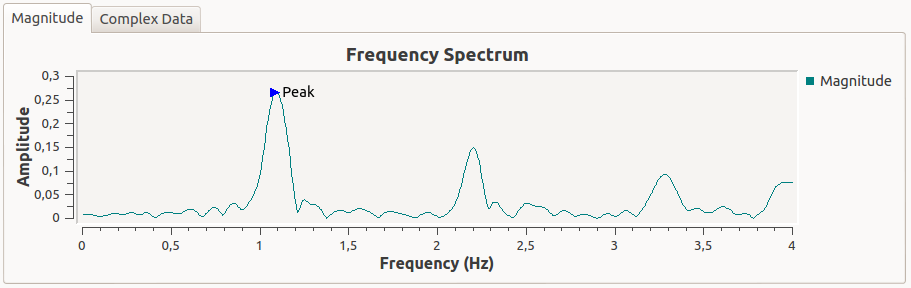
\includegraphics[width=350px]{images/withEverything.png}
	\caption{With everything}
	\label{fig:filter-window}
\end{figure}

\subsection{Zero Padding}
\label{subsec:zp}
Before applying the FFT, additional zeros are added to the input signal. This is a trick to interpolate the resulting frequency spectrum and make the possibility higher, that a real maximum is at an output frequency index. With this interpolating technique, the frequency resolution can be increased. Without zero padding, the frequency spectrum would look like displayed in figure \ref{fig:without-zp}.

\begin{figure}[H]
	\centering
	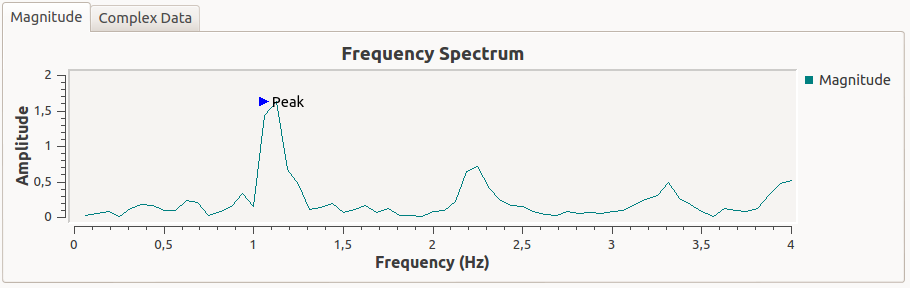
\includegraphics[width=350px]{images/noZeroPaddingAndWithEverythingElse.png}
	\caption{Without zero padding}
	\label{fig:without-zp}
\end{figure}

\subsection{FFT}
After using the filter, window function and zero padding, the FFT can be applied  to transform the data into the frequency domain. This is done by the FFTW library. The input data is the discrete light data array with N values. Because the discrete complex FT (DFT) works with complex numbers, the imaginary part of each input element is set to 0. The output of the FFT is also an array of N complex numbers.

\subsection{Converting/Scaling}
The resulting frequency domain values need to be scaled, to represent the correct amplitude. This is made by the following code snippet. The values are multiplied with $2$, because only the positive frequencies are used, but the complex DFT calculates positive and negative frequencies. Additionally, the values are brought to a more human readable format. The original complex numbers (sin and cos) in rectangular coordinate are converted to polar form with magnitude and phase shift. To apply the scaling, at first the correct values to scale need to be determined: The output format of the FFT is displayed in the following figure \ref{fig:output-format}. The first element of the array represents the DC offset (y-axis shift) and is not required. This is because this value changes based on the noise/environment light and is not needed to determine the heart rate. The next $[1, N/2]$ values represent the positive frequencies. The other values the negative frequencies. For this application, only the positive frequencies are used. So only the first half elements $[1, N/2]$ need our attention. Only the magnitude of this data is relevant, to calculate the heart rate. The phase shift is not of interest.

\begin{lstlisting}[caption=FFT.c]
double scaledAmplReal = 2 * out[i][0] / N;
double scaledAmplImag = 2 * out[i][1] / N;
// To polar coordinates magnitude
double magnitude = (sqrt(pow(scaledAmplReal, 2) + pow(scaledAmplImag, 2)));
\end{lstlisting}

\begin{figure}[H]
	\centering
	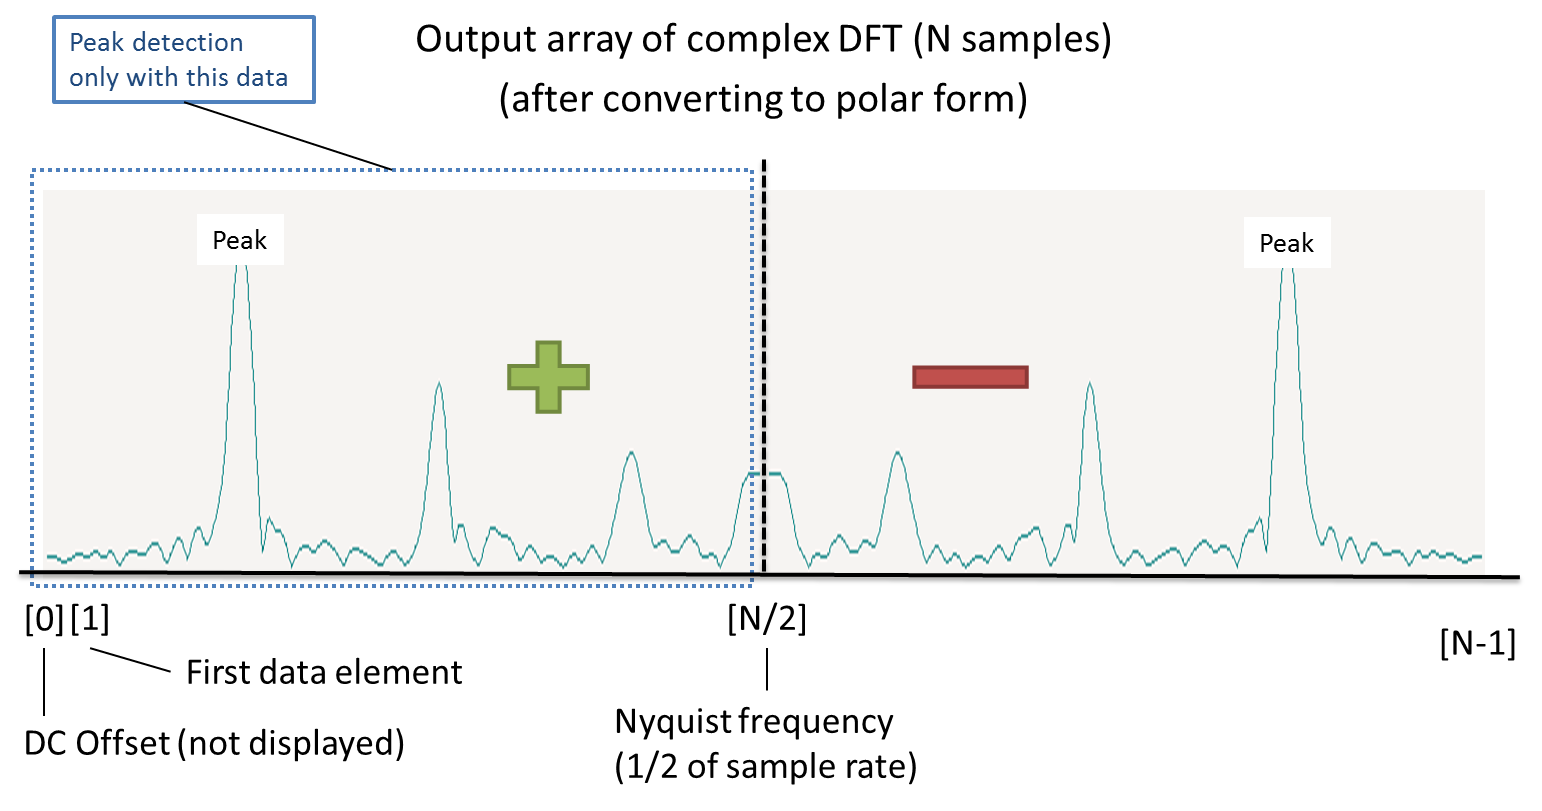
\includegraphics[width=350px]{images/outputFormat.png}
	\caption{Complex DFT output format}
	\label{fig:output-format}
\end{figure}

Additionally to the values of the y-axis, the x-axis need to be brought in the correct form. These values can be displayed as array indices, as fractions of the sample rate or as frequency. The most human readable format is the frequency representation. To calculate the available frequencies it is required to know the used sample rate. The frequency for a given array index $x$ is calculated with the following formula.

\begin{equation}
f(x) = f_{sample} * (x / N_{total})
\end{equation}

$N_{total}$ is the number of all samples including the zero padded ones. $f_{sample}$ is the sample rate in Hz.

\subsection{Peak Detection}
The last step to do is to detect the peak. This is done by iterating through the magnitude values and find the value (x-value/frequency) with the highest amplitude. This x-value needs to be converted into beats per minute (bpm), the standard heart rate unit.

\subsection{Parameter}
Additionally to applying the different signal processing steps, the correct parameter need to be chosen. There are several requirements to the signal processing:

\begin{itemize}
	\item{Small number of samples used for FFT (else it will take long time until enough data is gathered)}
	\item{High frequency resolution (0.1bpm)}
	\item{Fast calculation (for implementing on smart-phone/uC/...)}
	\item{Nice output data in frequency domain which allows easy peak detection}\\
\end{itemize}

All FFT parameter are saved in the structure \lstinline{FFT_properties}. The most important parameter are explained in the following sections.

\begin{lstlisting}
struct FFT_properties {
    int numberOfSamples = 0;
    int zeroPaddingSamples = 0;
    int totalSamples = 0; // N (numberOfSamples + zeroPaddingSamples)
    int outputSize = 0; // totalSamples / 2
    int slidingWindow = 0;

    double sampleInterval = 0.0; // delta x
    double sampleRate = 0.0; // Hz

    double segmentDuration = 0.0; // ms
    double frequencyResolution = 0.0; // Hz
    double frequencyResolutionWithZeroPadding = 0.0; // Hz
};
\end{lstlisting}

\subsubsection{Sample Rate}
To detect frequencies up to 4Hz, a minimal sample rate of 8Hz (according to the Shannon-Nyquist theorem) is required. This means at least a sample interval of 125ms is needed. The light sensor allows sample intervals up to 15ms.

\subsubsection{Frequency Resolution}
An optimal value for the number of samples are 128. It allows a good trade-off between frequency resolution and required sample time. However, the frequency resolution is not good enough (3.75bpm). To further improve the resolution, the following steps can be made:

\begin{itemize}
	\item{More samples (unsuitable, because requires more time)}
	\item{Zero Padding (interpolating by adding zeros to the end of the input data). However, its only a trick, because it adds not more information to the data.}
	\item{Higher sample rate. A higher sample rate results in more frequencies that can be detected. The filter can remove them.}
\end{itemize}

For getting a higher frequency resolution, zero padding is applied as explained in section \ref{subsec:zp}.

\subsubsection{Sliding Window}
\label{subsubsec:sliding-window}
To get fast new frequency spectra, the FFT is applied to the 128 samples every 5 samples. This is called segment duration/sliding window. It means, that every 5 samples, the FFT of the last 128 samples is calculated and should not be confused with the window function. The segment duration of 5 is trade off between fast results and required computation time. Else, the user would have wait 128 samples (= 16s) until he gets a new frequency spectrum and therefore the heart rate. To implement this, a special buffer (\ref{subsec:fft-buffer}) was created, which allows using different segment durations and fast data acquiring. Figure \ref{fig:sliding-window} shows the sliding window at three different times (t\_1, t\_2, t\_3).

\begin{figure}[H]
	\centering
	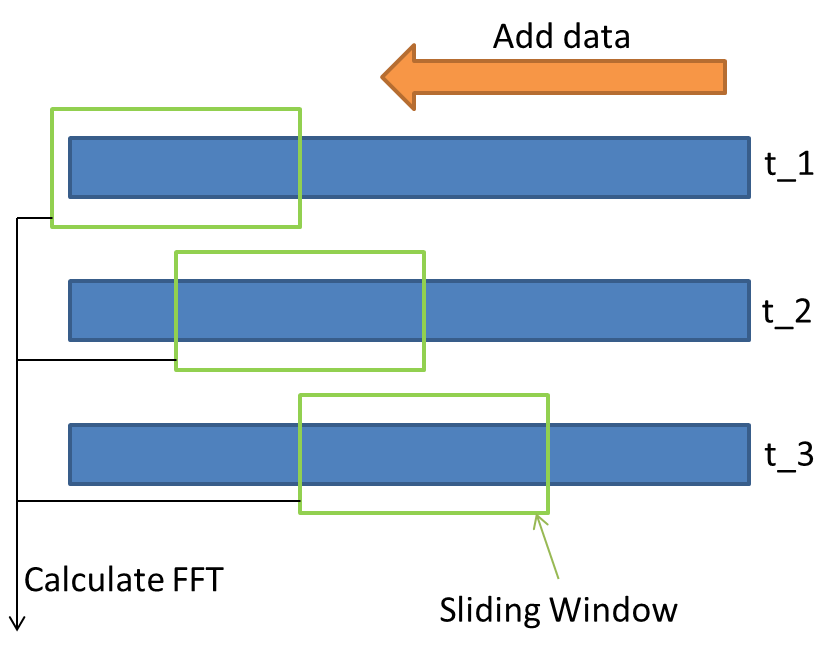
\includegraphics[width=200px]{images/slidingWindow.png}
	\caption{Sliding Window}
	\label{fig:sliding-window}
\end{figure}

\section{Results}
Figure \ref{fig:result} shows the final output signal.

\begin{figure}[H]
	\centering
	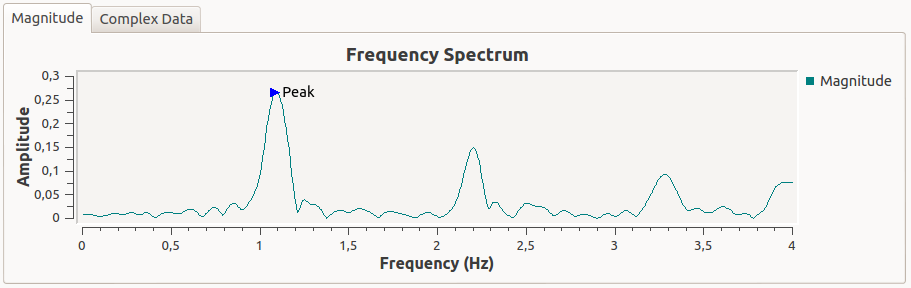
\includegraphics[width=350px]{images/withEverything.png}
	\caption{Final Result}
	\label{fig:result}
\end{figure}

The different peaks are the multiples of the fundamental frequency - the harmonic frequencies. The fundamental frequency is at $x = 1.1$ (1. harmonic), the 2. harmonic is at $2*x$, the 3. harmonic at $3*x$, ... . 

\chapter{Critique and Improvements}
The prototype is able to detect the heart rate with a very high precision (0.1 to 0.5bpm). Tests with commercial devices verified its functionality. Most commercial devices only have a resolution of 1bpm. Although HRM works very good, there can be still some improvements be made. Based on this prototype, more projects can be realised, to improve the heart rate monitor.

\begin{itemize}
	\item{Porting to an Arduino}
	\subitem{- FFT library is available}
	\subitem{- Performance tests need to be made}
	\item{Using a smart-phone for signal processing}
	\item{Porting to a smaller uC.}
	\item{Adding a Bluetooth module (trivial)}
	\item{Add oxygen saturation measurement}
	\subitem{- Easy to implement with the existing knowledge}
	\item{Create a wrist band (with better environment light shielding)}
	\item{Brighter LED}
	\item{Better light sensor (more sensitive - new version is available)}
	\item{Do additional tests with different mounting possiblities (reflection, hand wrist, ...)}
\end{itemize}

Figure \ref{fig:data-flow1} shows a hardware setup with a Bluetooth module, to allow wireless heart rate detection. As shown in the picture, the heart rate should be calculated on the Arduino. Only the calculated heart rate is sent via Bluetooth to the user.

\begin{figure}[H]
	\centering
	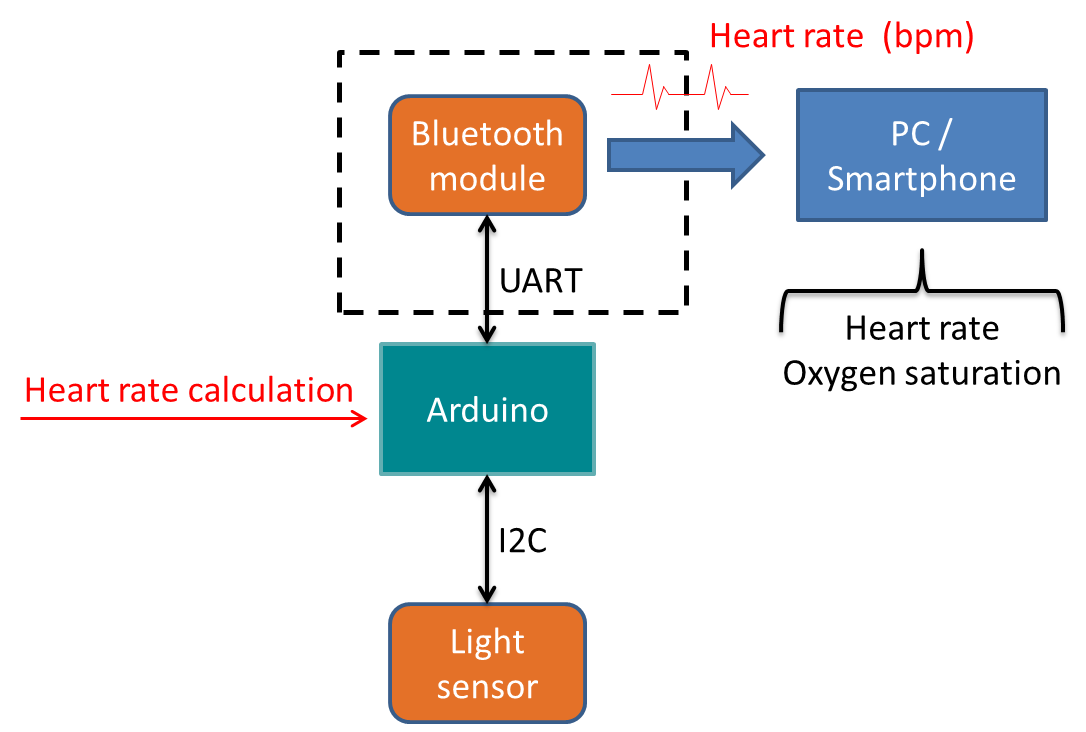
\includegraphics[width=350px]{images/general_dataFlow_first.png}
	\caption{Project Setup}
	\label{fig:data-flow1}
\end{figure}

\chapter{Implementation Details}
\label{chap:impl-details}
This chapter describes the most important implementation details. For further information and API documentation, a doxygen file is available.

\section{Software}
\subsection{Graphical User Interface}
The GUI is used for displaying the different parameter and data. Additionally it calls the signal processing module. Using a GUI simplifies the debugging and optimization process. In this chapter, the usage of the signal processing module from the GUI is covered.

\begin{figure}[H]
	\centering
	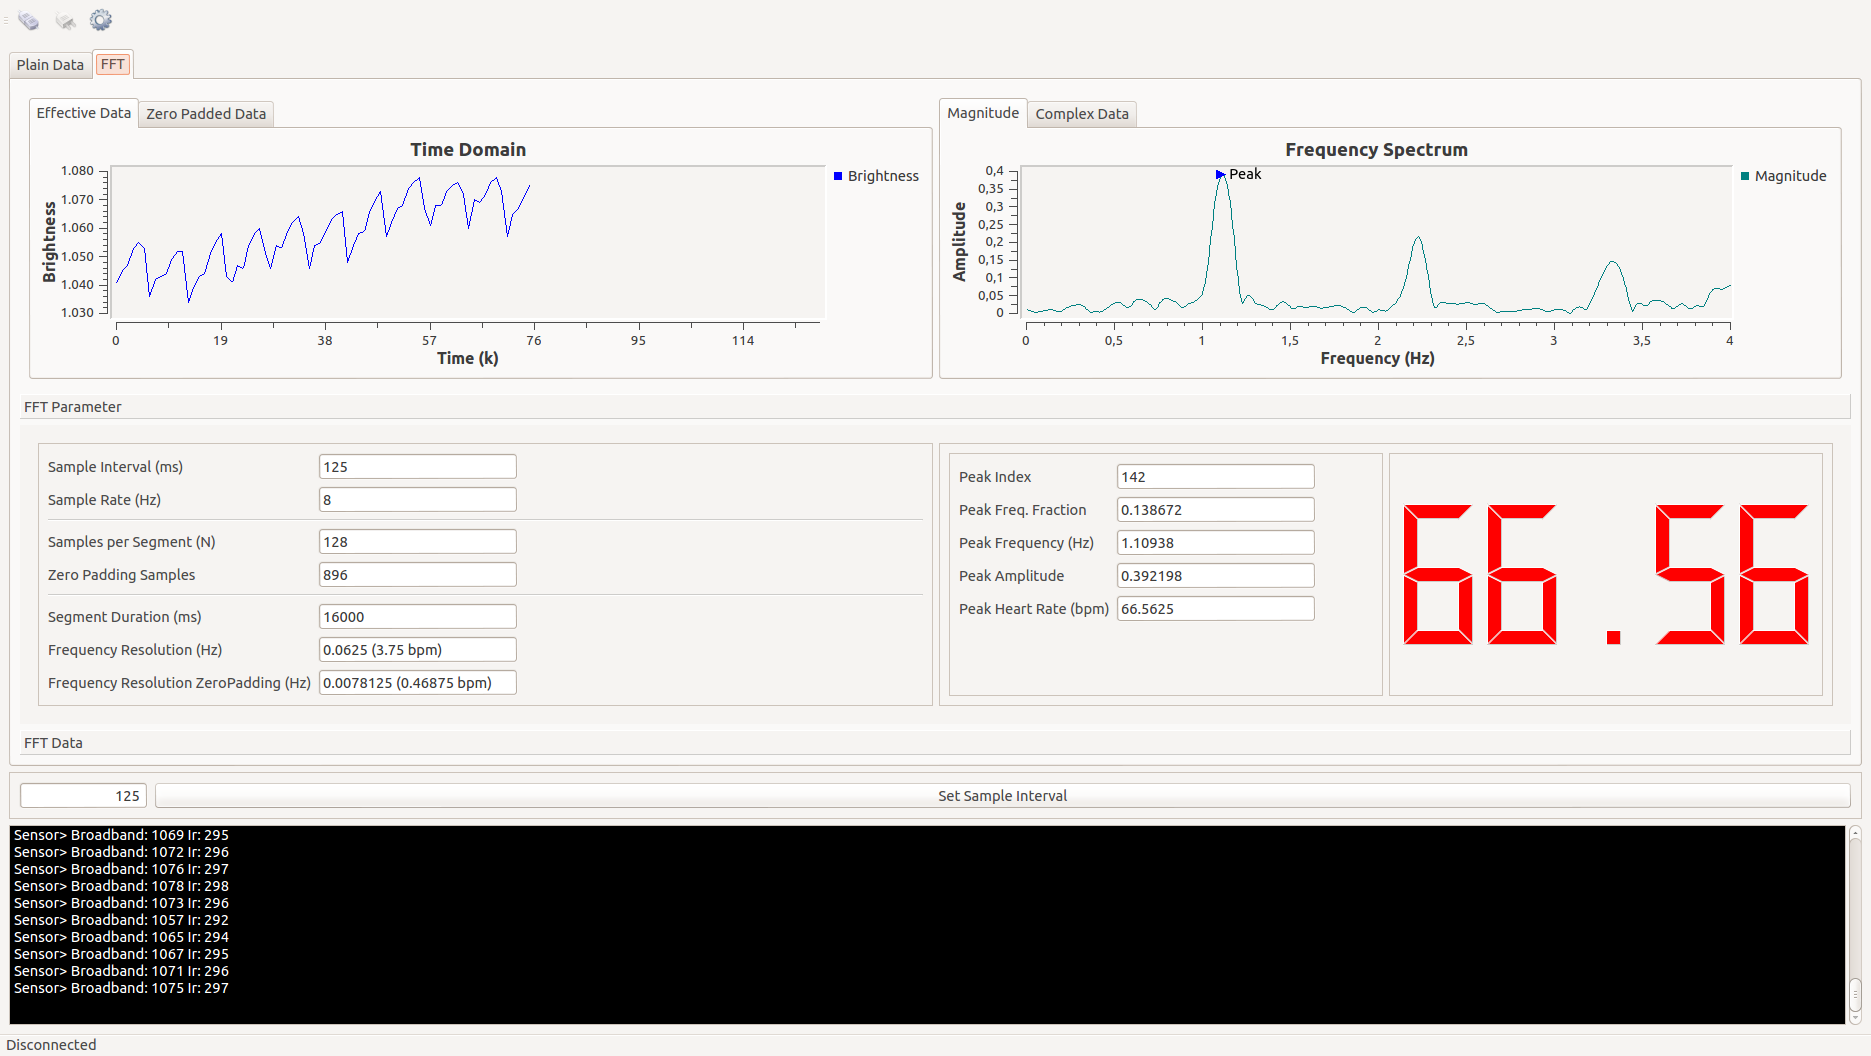
\includegraphics[width=400px]{images/screen2.png}
	\caption{GUI}
	\label{fig:gui}
\end{figure}

\begin{lstlisting}[caption=MainWindow.cpp]
if (fft.addSample(data.broadband))
	displayFrequencies();
\end{lstlisting}

\lstinline{fft.addSample()} is called in the \lstinline{receiveSensorData()} slot (when sensor data is received). When it returns non-zero, the DFT of the last sliding window was calculated. The Function \lstinline{displayFrequencies()} is called:

\begin{lstlisting}[caption=MainWindow.cpp]
double *magnitude = fft.getMagnitude();
double *real = fft.getRealPart();
double *imaginary = fft.getImaginaryPart();

FFT_properties properties = fft.getProperties();

// Max peak
int indexMax = fft.getPeak();
displayPeak(indexMax, magnitude[indexMax]);

// Display properties ...
// Display output data ...
\end{lstlisting}

In rows 1-3 the frequency spectrum's magnitude (polar coordinate) and real/imaginary values (rectangular coordinates - for debugging) are queried. After that, the current properties are saved in a \lstinline{FFT_properties} structure. The peak index of the frequency spectrum is computed with \lstinline{getPeak()}.

\subsection{Serial Interface}
The class \lstinline{Serial.h} receives UART data from the Arduino and saves it in the structures \lstinline{SensorData} and \lstinline{SensorSettings} for easier usage. It parses the incoming commands and converts it to data structures which are easier to interpret. The following signals are available for receiving plain string data, the light sensors luminosity values or its settings.

\begin{lstlisting}
signals:
    void receiveLine(QString data);
    void receiveSensorData(SensorData data);
    void receiveSensorSettings(SensorSettings settings);
\end{lstlisting}

The sensor settings are saved in the following struct.

\begin{lstlisting}
struct SensorSettings {
    QString sensor;
    QString id;
    QString max; // Max luminosity value
    QString min; // Min luminosity value
    QString resolution;
    QString sampleInterval;
};
\end{lstlisting}

The light sensor data (broadband and infra-red) are saved in the \lstinline{SensorData} structure.

\begin{lstlisting}
struct SensorData {
	uint16_t broadband;
	uint16_t ir;
};
\end{lstlisting}

Sending data to the Arduino is done with the \lstinline{sendData(QString string)} function.

\subsubsection{Serial Configuration}
The following serial port configuration is used:
\begin{itemize}
	\item{Port Name: /dev/ttyACM0}
	\item{Baudrate: 9600}
	\item{Data Bits: 8}
	\item{Parity: No}
	\item{Stop Bit: 1}
	\item{Flow Control: No}
\end{itemize}

\subsection{FFTBuffer}
\label{subsec:fft-buffer}
The class \lstinline{FFTBuffer.h} is a wrapper for FFTWs own buffer (\lstinline{fftw_complex} array). Because the FFTW data buffer is only an array and does not allow more comfortable container operations this wrapper class was written. With this class, data can be added like it would be a queue. Optional, zero padding can be enabled. The following variables are used, to configure the size of the buffer:

\begin{lstlisting}
int effectiveSize;
int zeroPadSize;
// effectiveSize + zeroPadSize = totalSize
int windowSize;
\end{lstlisting}

\lstinline{effectiveSize} is the number of data samples the buffer can have as a maximum. After \lstinline{effectiveSize} samples were added, the FFT of this data can be calculated. \lstinline{zeroPadSize} defines how much additional elements are optionally used for zero padding. \lstinline{windowSize} is the size of the sliding window explained in \ref{subsubsec:sliding-window}. For basic usage the function \lstinline{add()} is used:

\begin{lstlisting}
fftw_complex *add(double p_data);
\end{lstlisting}

This function adds the parameter \lstinline{p_data} as real value to the data vector. The imaginary part is set to zero. It returns \lstinline{nullptr} if the desired maximum capacity is not reached. If it returns non-zero, a pointer to the \lstinline{fftw_complex} array with valid data is returned. Internally, the data is first copied to a vector container. After \lstinline{effectiveSize} is reached, the data is copied to the \lstinline{fftw_complex} array. After copying, zero padding is applied. If the sliding window is enabled, \lstinline{(effectiveSize - windowSize)} elements are preserved in the data vector. \lstinline{windowSize} new elements are required until \lstinline{add()} returns the next array pointer. Figure \ref{fig:fft-buffer} shows the internal work flow.

\begin{figure}[H]
	\centering
	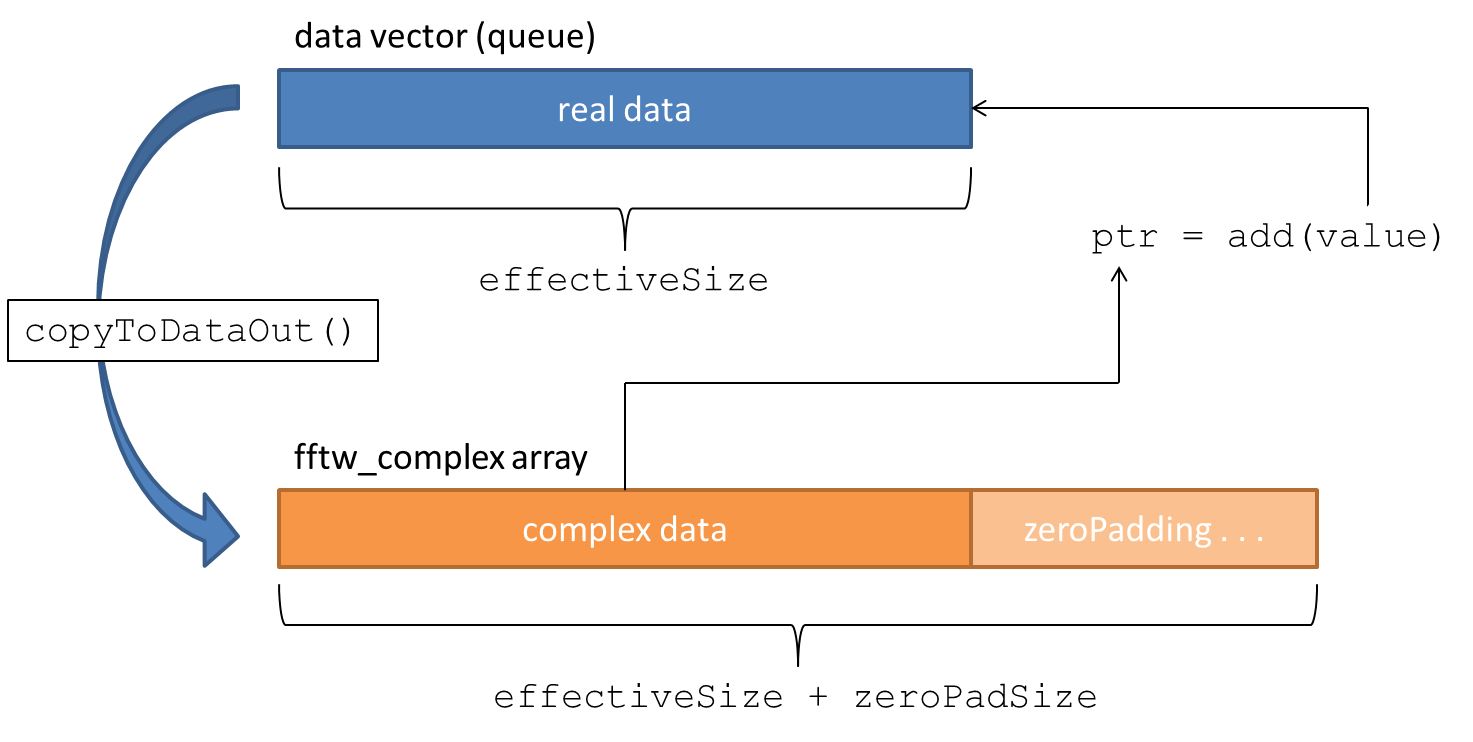
\includegraphics[width=300px]{images/FFTBuffer.png}
	\caption{FFTBuffer}
	\label{fig:fft-buffer}
\end{figure}

More functions are supported, to set or get specific elements or get the different sizes.

\subsection{FFT}
The class \lstinline{FFT} is the main part of HRM and does the signal processing. When enough data was aquired to calculate the DFT, the following steps are executed:

\begin{lstlisting}[caption=FFT.c]
// Functions for input time domain.
filter();
windowFunction();

fftw_execute(plan);

// Function for output frequency domain.
scaleAndConvert();
\end{lstlisting}

\lstinline{filter()} convolutes the input signal with the butterworth bandpass filter and cuts the stabilization time. \lstinline{windowFunction()} applies the Hamming-Window. After calcualting the DFT with \lstinline{fftw_execute(plan)} the resulting frequency spectrum is correctly scaled (to get correct amplitude values) and converted to polar coordinates (\lstinline{scaleAndConvert()}). As a result of these steps, the output data is available through the following pointers:

\begin{lstlisting}[caption=FFT.c]
double *outMagnitude;
double *outReal;
double *outImaginary;
\end{lstlisting}

\lstinline{outMagnitude} consists of the magnitude part from the converted polar coordinates, \lstinline{outReal} and \lstinline{outImaginary} are the real and imaginary parts of the output from the rectangular coordinates. All arrays have $N/2$ elements. The output data is converted in the following way:

\begin{lstlisting}[caption=FFT.c]
// Complex value to magnitude
// (multiply with 2 because of the negative and positive frequencies)
double scaledAmplReal = 2 * out[i][0] / N;
double scaledAmplImag = 2 * out[i][1] / N;
// To polar coordinates magnitude
double magnitude = (sqrt(pow(scaledAmplReal, 2) + pow(scaledAmplImag, 2)));

outReal[i-1] = scaledAmplReal;
outImaginary[i-1] = scaledAmplImag;
outMagnitude[i-1] = magnitude;
\end{lstlisting}

The array index of the peak value of the magnitude data to get the heart rate can be requested with the function \lstinline{int getPeak()}. For calculating the FFT with the function \lstinline{fftw_execute(plan)} with the FFTW library, at first a plan has to be created. This is done in the \lstinline{FFT} class constructor. The most important parameter are the first three: Size of the buffer, input buffer and output buffer.

\begin{lstlisting}[caption=FFT.c]
plan = fftw_plan_dft_1d(buffer->totalSize(), buffer->get(), out, FFTW_FORWARD, FFTW_MEASURE | FFTW_PRESERVE_INPUT);
\end{lstlisting}

\subsection{Arduino Module}
The Arduino module software is required to get the light sensors values and send them via UART to the PC. Because this is its main functionality, the software is very small and does not require a lot of performance. The main loop is displayed in the following code snippet.

\begin{lstlisting}
void loop()
{ 
  luminosityManualTiming();
  
  readData();
}
\end{lstlisting}

The function \lstinline{readData()} reads incoming UART data and interprets it (for getting sensor settings or setting the sample interval/rate). The function \lstinline{luminosityManualTiming()} reads the sensor values with the extended manual timing driver functionality:

\newpage

\begin{lstlisting}
void luminosityManualTiming()
{
  uint16_t broadband, ir;
  
  tsl.beginIntegrationCycle();
  delay(sampleInterval);
  tsl.stopIntegrationCycle(&broadband, &ir);
  
  printLuminosity(broadband, ir);
}
\end{lstlisting}

The sample rate/interval is saved in the variable \lstinline{sampleInterval}, which can be set from the PC.

\subsection{Light Intensity Sensor}
This section describes the usage of the extended light sensor library.

\begin{lstlisting}[caption=Adafruit driver]
tsl.enableAutoRange(true);
tsl.setIntegrationTime(TSL2561_INTEGRATIONTIME_13MS);

uint16_t broadband, ir;
tsl.getLuminosity(&broadband, &ir);
\end{lstlisting}

Line 1 sets the gain value to auto range. That means it adapts automatically to the sensors environment. On line 2 the integration time is set to 13ms (low resolution, fast processing). Line 5 queries for the luminosity values of the broadband and ir photodiode. For the use in this project, the sensor driver had to be slightly modified to allow manual integration times. The original driver allows only to set three different static integration times (13ms, 101ms, 402ms). Specific integration time are required to allow the desired sample frequencies. The extended driver provides functions to start and stop the integration of the light values, shown in the following code extract.

\begin{lstlisting}[caption=Adafruit\_TSL2561\_U.h]
/* Manual timing control */
void beginIntegrationCycle();
void stopIntegrationCycle(uint16_t *broadband, uint16_t *ir);
\end{lstlisting}

\newpage

\section{Wiring}
\label{sec:wiring}
Figure \ref{fig:wiring} shows the wired luminosity sensor and the red LED. Only the actually parts required for the prototype are displayed. A picture of LED and sensor is displayed in figure \ref{fig:led-sensor}. The complete prototype installation is shown in \ref{fig:prototype}.

\begin{figure}[H]
	\centering
	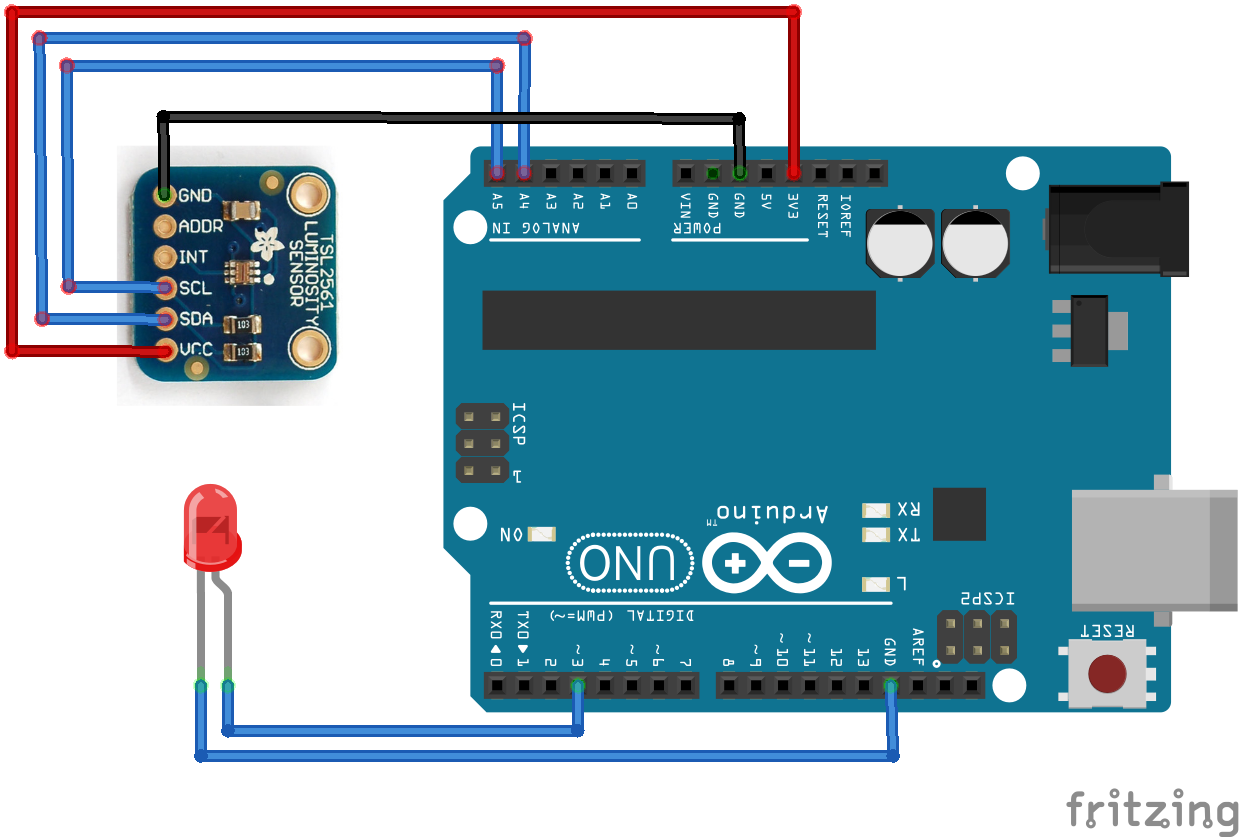
\includegraphics[width=300px]{images/wiring.png}
	\caption{Wiring}
	\label{fig:wiring}
\end{figure}

\begin{figure}[H]
	\centering
	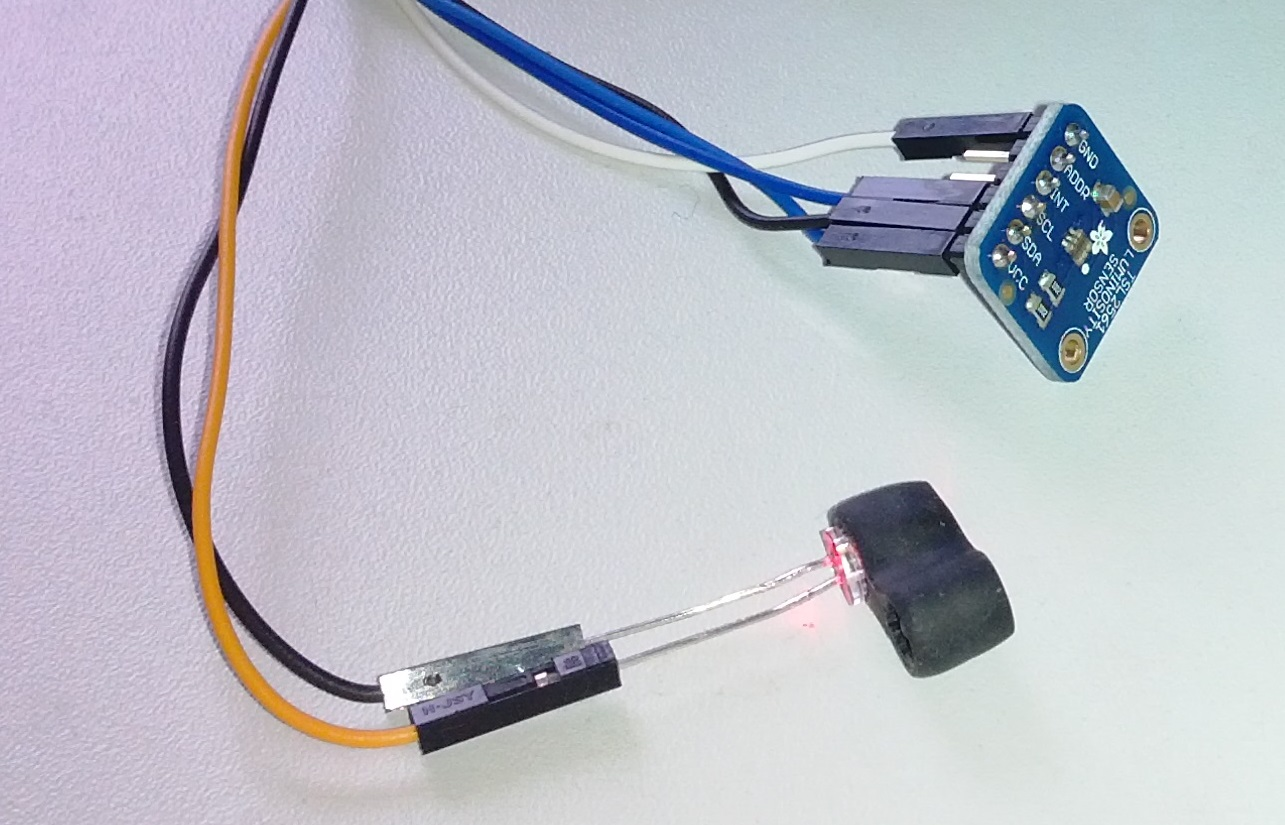
\includegraphics[width=300px]{images/ledAndSensor.jpg}
	\caption{LED and sensor}
	\label{fig:led-sensor}
\end{figure}

\begin{figure}[H]
	\centering
	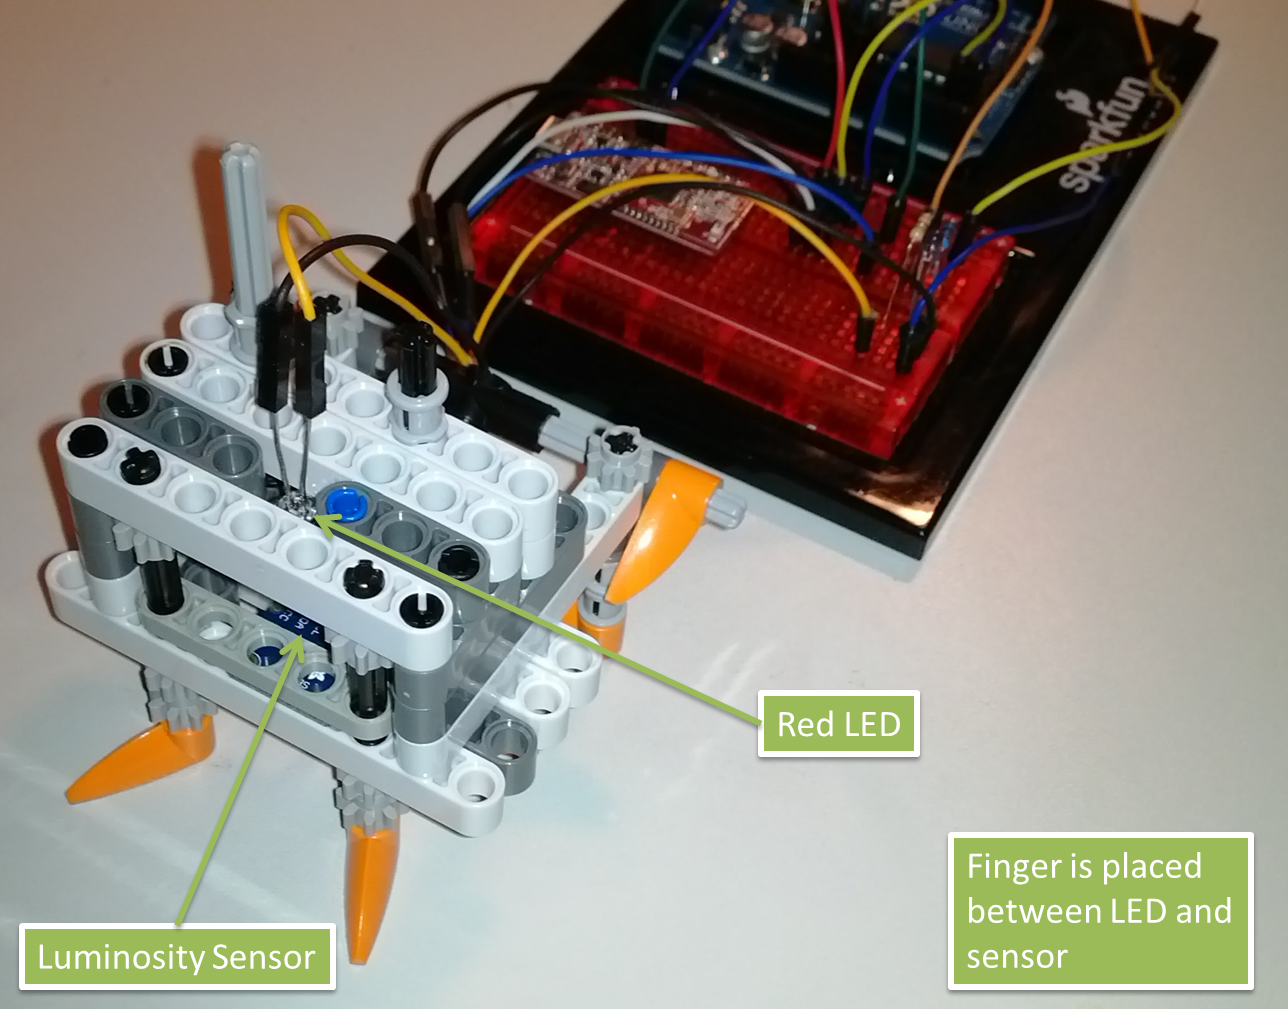
\includegraphics[width=300px]{images/prototype_labeled.png}
	\caption{Prototype}
	\label{fig:prototype}
\end{figure}

\section{Source Code}
The source code and the documentation are available at Github (\url{https://github.com/UbiquitousComputingSS14}). It is licensed under the GPLv3 license.

\begin{thebibliography}{999}
	\bibitem{bib:pulse-oximetry} Pulse Oximetry, Dr. Chloe Borton, \url{http://www.patient.co.uk/doctor/pulse-oximetry}, 30.05.2014
	\bibitem{bib:tsl-sensor} TSL2561, \url{https://learn.adafruit.com/tsl2561/overview}, 30.05.2014
	\bibitem{bib:arduino-board} Arduino Board, \url{http://www.adafruit.com/product/50}, 31.05.2014
	\bibitem{bib:bluetooth-adapter} Bluefruit EZ-Link, \url{https://learn.adafruit.com/introducing-bluefruit-ez-link/overview}, 31.05.2014
	\bibitem{bib:tsl-library} TSL 2561 Library, \url{https://github.com/adafruit/Adafruit_TSL2561}, 31.05.2014
	\bibitem{bib:sensor-library} Adafruit Unified Sensor Driver library, \url{https://github.com/adafruit/Adafruit_Sensor}, 31.05.2014
	\bibitem{bib:dpsguide} Steven W. Smith, Ph.D. ,\url{http://www.dspguide.com/}, 21.07.2014
	\bibitem{bib:amidror} Isaac Amidror, Springer, Mastering the Discrete Fourier Transform in One, Two or Several Dimensions - Pitfalls and Artifacts, 21.07.2014
	\bibitem{bib:neubauer} André Neubauer, Springer, DFT – Diskrete Fourier-Transformation, 21.07.2014
	\bibitem{bib:mertins} Alfred Mertins, Springer, Signaltheorie, 21.07.2014
	\bibitem{bib:thefourier} \url{http://www.thefouriertransform.com/series/fourier.php}
	\bibitem{bib:stanford} \url{https://ccrma.stanford.edu/~jos/mdft/}
	\bibitem{bib:bourke} \url{http://paulbourke.net/miscellaneous/dft/}
	\bibitem{bib:blog} \url{http://www.ignaciomellado.es/blog/Measuring-heart-rate-with-a-smartphone-camera}
	\bibitem{bib:filter} \url{http://www-users.cs.york.ac.uk/~fisher/mkfilter/trad.html}
\end{thebibliography}

\end{document}